%=============================================
%=============================================
%=============================================

\begin{frame}[fragile]

  {\Huge Kokkos Remote Spaces: Support for PGAS in Kokkos}

  \vspace{10pt}

  {\large How to write a PGAS application with Kokkos.}

  \vspace{20pt}

  \textbf{Learning objectives:}
  \begin{itemize}
    \item {How to create global Views.}
    \item {How access global data.}
    \item {Taking a closer look at SPMV (CG).}
  \end{itemize}

  \vspace{-20pt}

\end{frame}


%=============================================
%=============================================
%=============================================

\begin{frame}[fragile]{Remote Spaces: Motivation}
  \textbf{Previous Example: \texttt{Vector-Shift}}
  \vspace{12pt}
  \center
  \begin{center}
  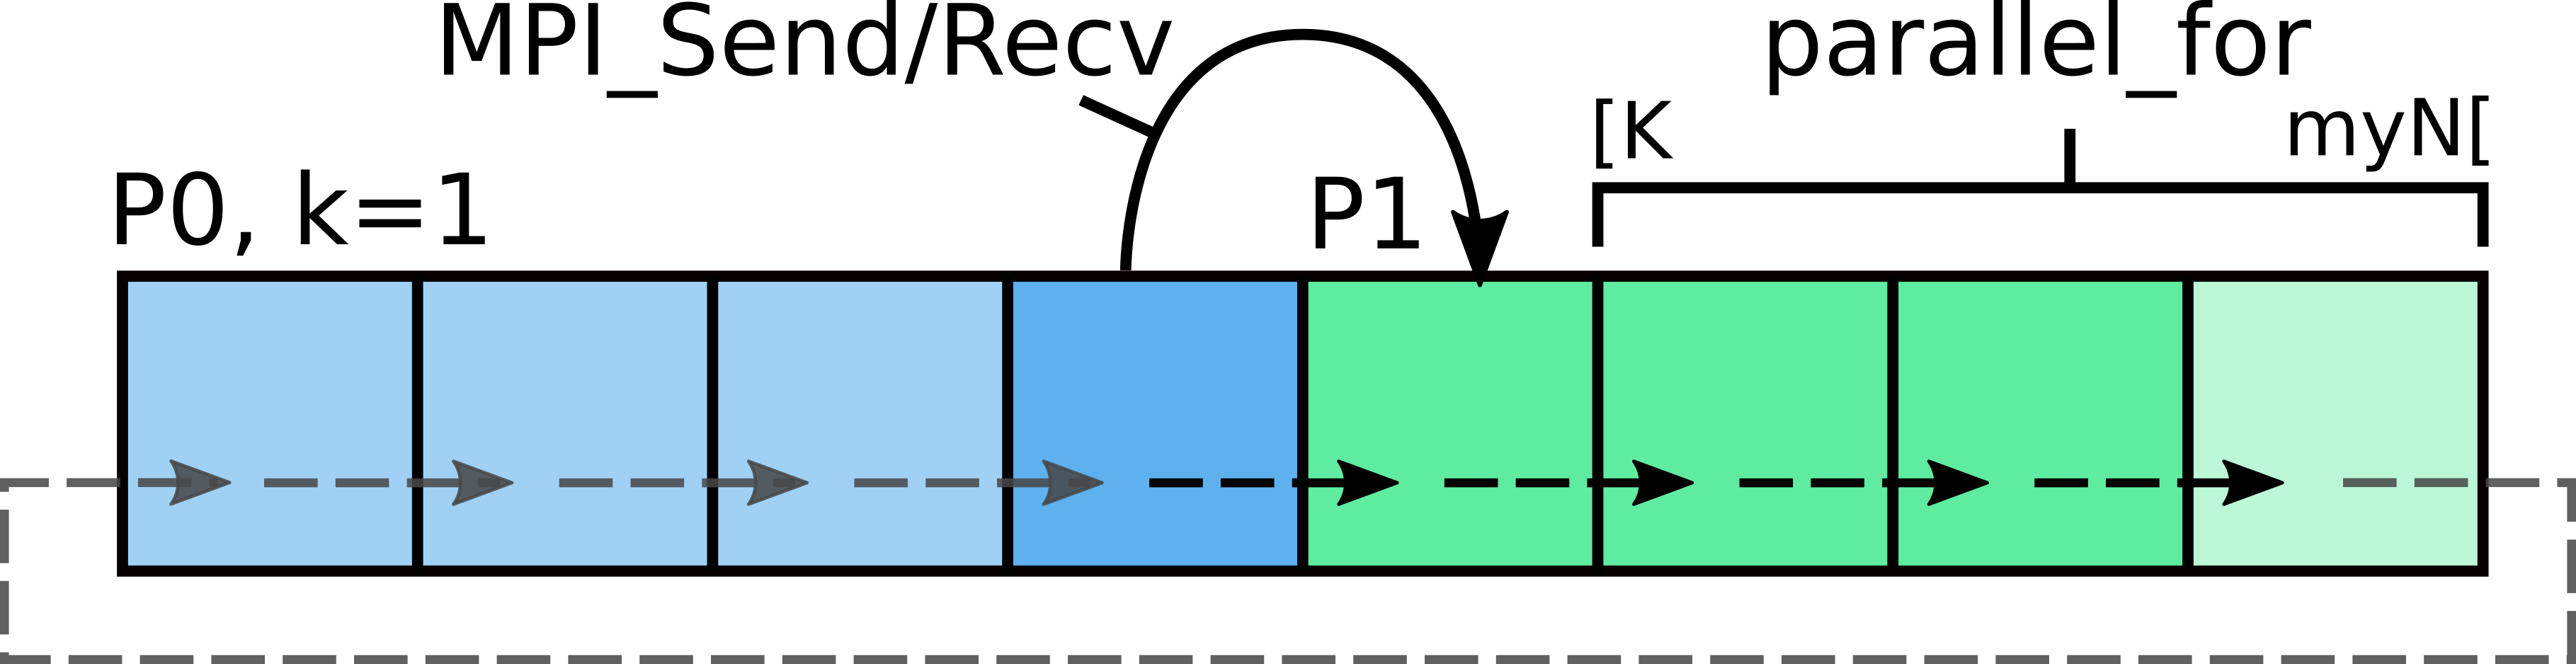
\includegraphics[width=0.50\textwidth]{figures/VectorShift}
  \end{center}
  \begin{code}[keywords={recv_ptr, send_ptr, send_view, recv_view,double,
  KOKKOS_LAMBDA,MPI_Irecv,MPI_Isend,parallel_for, MPI_Waitall}]
  auto send_view = Kokkos::subview(A,std::make_pair(myN-K, myN));
  auto recv_view = Kokkos::subview(B,std::make_pair(0, K));
  ...
  MPI_Request requests[2];
  MPI_Irecv(recv_ptr,recv_view.size(),MPI_DOUBLE,
            source,1,MPI_COMM_WORLD,&requests[0]);
  MPI_Isend(send_ptr,send_view.size(),MPI_DOUBLE,
            target,1,MPI_COMM_WORLD,&requests[1]);
  parallel_for("Shift",RangePolicy<>(K,myN), 
    KOKKOS_LAMBDA(int i) { B(i) = A(i-K); });
  MPI_Waitall(2,requests,MPI_STATUSES_IGNORE);
  \end{code}
  \begin{itemize}
    \item \textbf{How to simplify communication, and reduce host-device data movement?}
    \end{itemize}
\end{frame}

%=============================================
%=============================================
%=============================================

\begin{frame}[fragile]{Remote Spaces: The PGAS Model}
  \vspace{15pt}
  \textbf{PGAS (Partitioned Global Address Space)}
  \begin{center}
    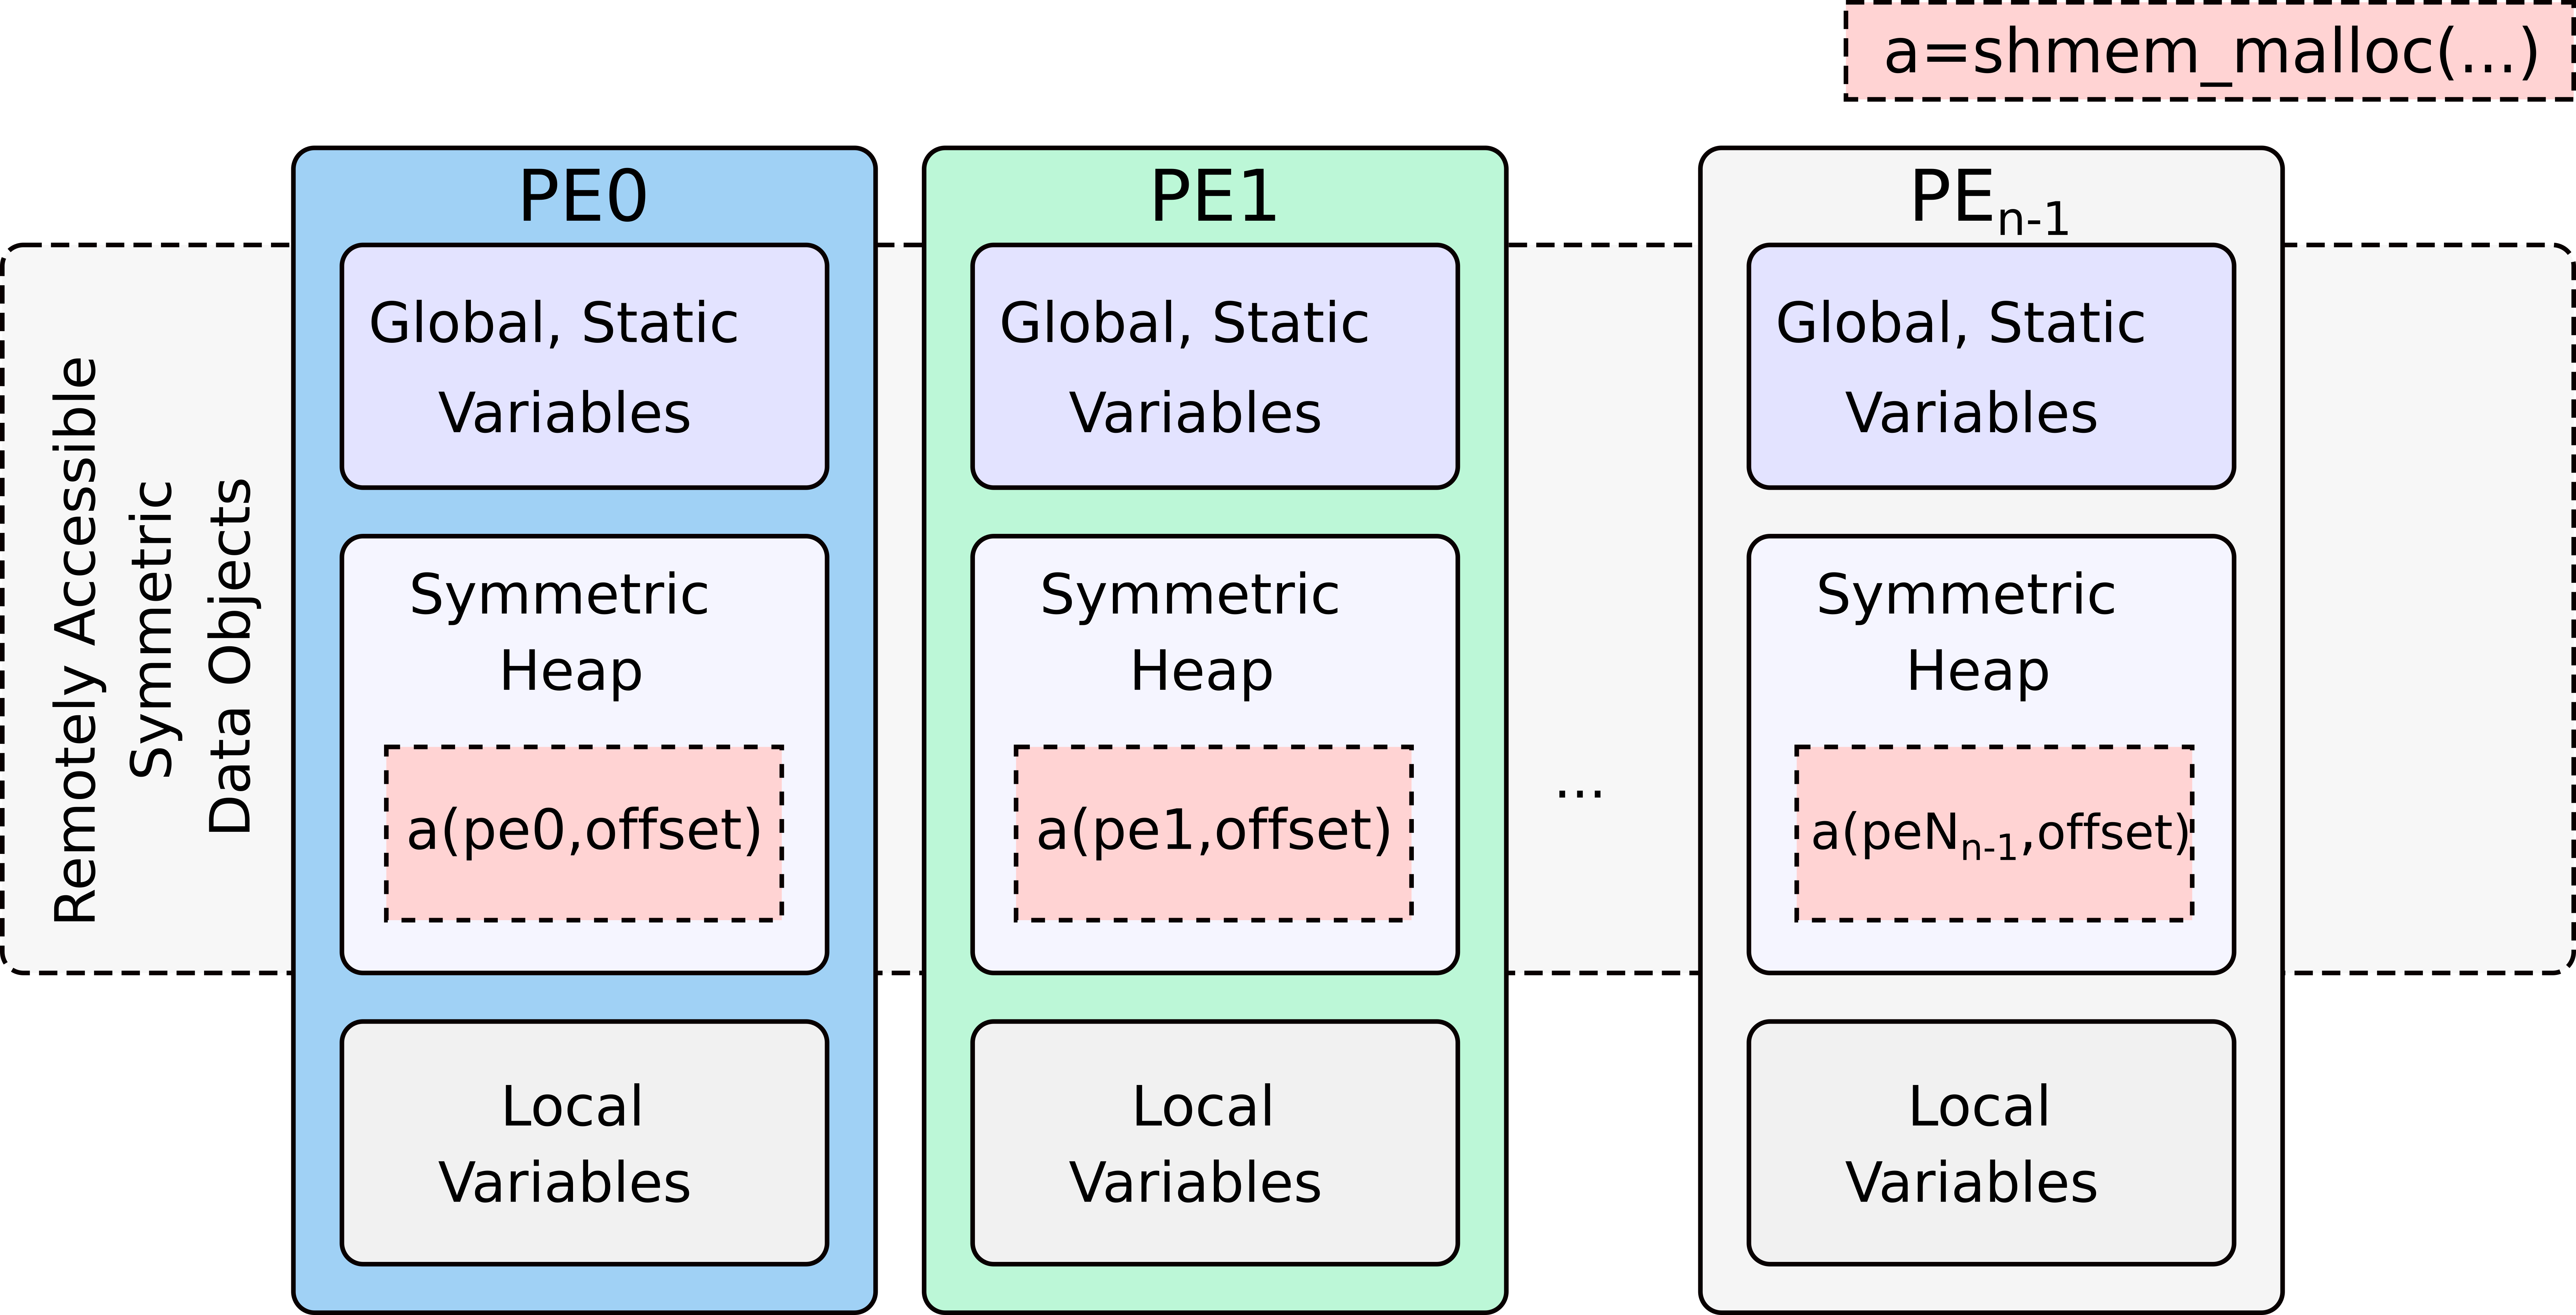
\includegraphics[width=0.8\textwidth]{figures/PGAS2}
  \end{center}
  \begin{itemize}
    \item Variable \texttt{a} is globally accessible through \texttt{Put} and \texttt{Get} operations,
    \texttt{PE} and \texttt{Offset} are used for global addressing.
    %\end{itemize}
  \end{itemize}
\end{frame}

%=============================================
%=============================================
%=============================================

\begin{frame}[fragile]{Remote Spaces: The PGAS Model}
  \vspace{10pt}
  \textbf{Different implementations, same conceptual API}
  \begin{itemize}
    \item OpenSHMEM
    \begin{itemize}
    \item void *shmem\_malloc(size\_t size);
    \item void shmem\_T\_p(T *dest, T value, int pe);
    \item TYPE shmem\_T\_g(T *src, int pe);
    \end{itemize}
    \item NVSHMEM
    \begin{itemize}
    \item void *nvshmem\_malloc(size\_t size);
    \item void nvshmem\_T\_p(T *dest, T value, int pe);
    \item TYPE nvshmem\_T\_g(TYPE *srct, int pe);
    \end{itemize}
    \item MPI One-Sided
    \begin{itemize}
    \item int *MPI\_Win\_allocate(size\_t size);
    \item int MPI\_Put(T *src, int count, MPI\_TYPE, int target\_pe,...);
    \item int MPI\_Get(T *target, int count , MPI\_TYPE, int source\_pe,...);
    \end{itemize}
  \end{itemize}
\end{frame}

%=============================================
%=============================================
%=============================================

\begin{frame}[fragile]{Remote Spaces: Namespace and API}
  \vspace{10pt}
  \textbf{Programming with Kokkos Remote Spaces: Vector Shift}
  \begin{itemize}
    \item Allocate a remote View
  \end{itemize}
  %\vspace{2pt}
  \begin{code}[keywords={RemoteSpace_t,RemoteView_t,Kokkos,View}]
  using RemoteSpace_t = Kokkos::Experimental::SHMEMSpace;
  Kokkos::View<T**,RemoteSpace_t> a("A",numPEs,myN);
  \end{code}
  %=============================================
  \pause
  \begin{itemize}
    \item Access global memory 
  \end{itemize}
  %\vspace{2pt}
  \begin{code}[keywords={RemoteSpace_t,RemoteView_t,Kokkos,View}]
  a(0,0) = 6; //Writes 6 to view a on PE 0 at offset 0
  a(1,8) = 3; //Writes 3 to view a on PE 1 at offset 8
  \end{code}
  %=============================================
  \pause
  %\vspace{2pt}
  \begin{itemize}
    \item Fence
  \end{itemize}
  \begin{code}[keywords={}]
  RemoteSpace_t().fence(); 
  \end{code}  
  %=============================================
    \pause
  %\vspace{2pt}
  \begin{itemize}
    \item Copy data to other memory space
  \end{itemize}
  \begin{code}[keywords={RemoteSpace_t,RemoteView_t,Kokkos,View,Experimental,deep_copy}]
  Kokkos::View<T**,Kokkos::HostSpace_t> a_h("A_h",1,myN);
  Kokkos::Experimental::deep_copy(a_h,a);
  \end{code}  
  %=============================================
\end{frame}

%=============================================
%=============================================
%=============================================

\begin{frame}[fragile]{Remote Spaces: Namespace and API}
  \vspace{10pt}
  \textbf{Vector Shift with Kokkos Remote Spaces}
    \vspace{4pt}
  \center
  \begin{center}
  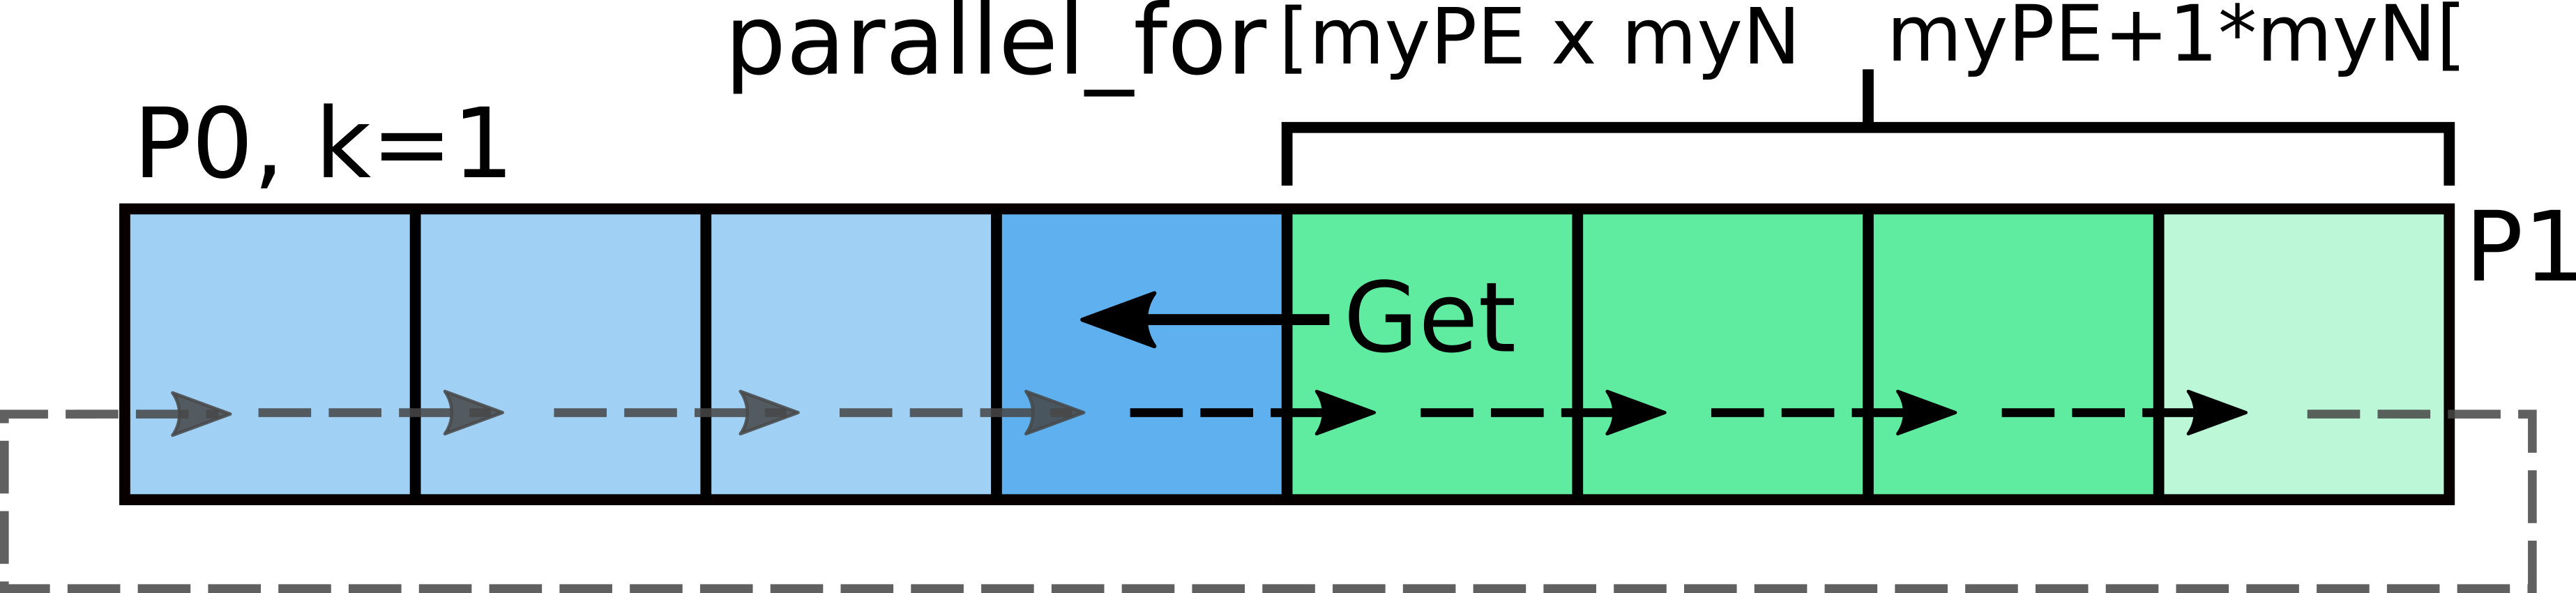
\includegraphics[width=0.50\textwidth]{figures/VectorShiftPGAS}
  \end{center}\
  \vspace{10pt}
  \begin{code}[keywords={RemoteSpace_t,RemoteView_t,parallel_for,Kokkos,View,Experimental,deep_copy, RangePolicy, KOKKOS_LAMBDA}]
  RemoteView_t a("A",numPEs,myN);
  RemoteView_t b("B",numPEs,myN);

  Kokkos::parallel_for("Shift",Kokkos::RangePolicy<>
  (myPE*myN,(myPE+1)*myN), KOKKOS_LAMBDA(const int i) { 
    int j = i+k; //Shift
    b((j/myN)%numPEs, j%myN) = a(myPE, i);
  });

  RemoteSpace_t().fence(); 
  \end{code}
\end{frame}

%=============================================
%=============================================
%=============================================

\begin{frame}[fragile]{Sparse Communication Patterns}
  \textbf{Example Sparse Matrix Multiply $y = A*x$:}
  Sparse Matrix Representation in Compressed Row Storage (CRS):
  \begin{itemize}
    \item Store non-zero matrix elements sorted by occurence.
    \item Store the actual column index of each value.
    \item Store the offsets of where each row begins.
  \end{itemize}
  \vspace{3pt}
  %=============================================
  \pause
    \textit{Single Node Implementation:}
    \begin{code}[keywords={for,RemoteSpace_t,RemoteView_t,parallel_for,Kokkos,View,Experimental,deep_copy,RangePolicy, KOKKOS_LAMBDA}]
      Kokkos::parallel_for("SPMV",nrows, KOKKOS_LAMBDA(int row) {
      for(j=A.row_offset(row); j< A.row_offset(row+1); j++)
      y(row) += A.val(j)* x(A.idx(j));
      });
    \end{code}\\
  %=============================================
  \pause

    \begin{columns}[t,onlytextwidth]
    \column{.7\textwidth}
     How to distribute data:
    \begin{itemize}
       \item The matrix is distributed by rows.
       \item The vectors are distributed by elements.
    \end{itemize}
    \textbf{Problem:$A.idx(j)$ may be on a remote node!}
    \column{.3\textwidth}
    \begin{center}
      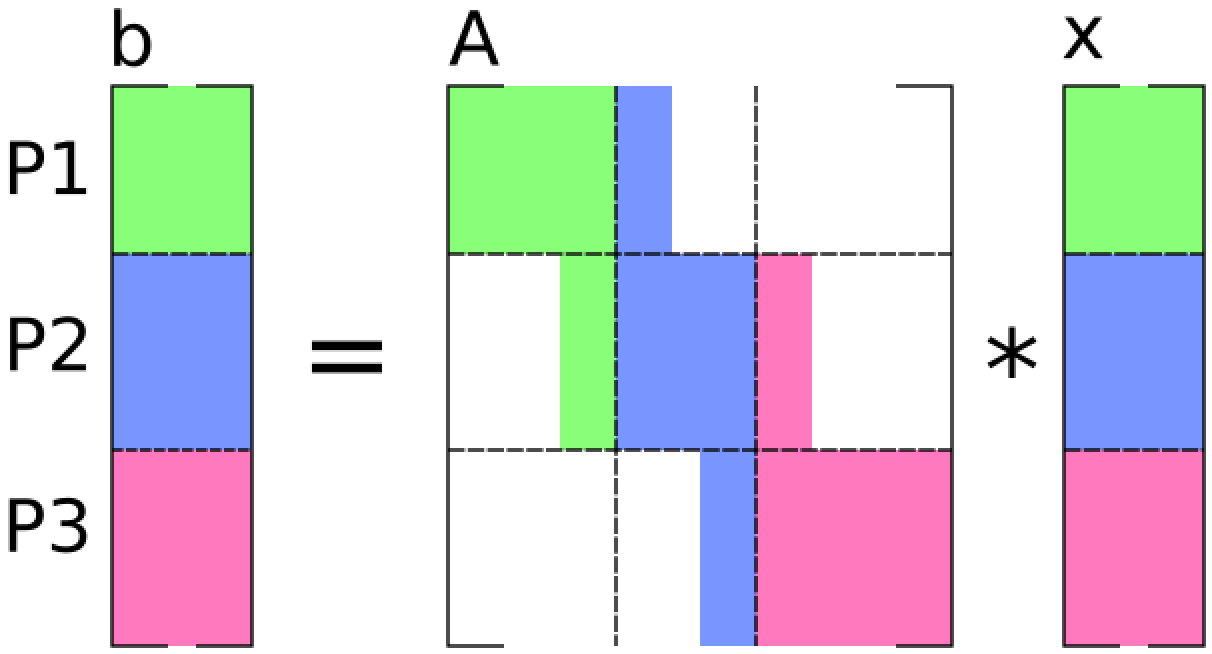
\includegraphics[width=1\textwidth]{figures/MatVecPGAS}
    \end{center}
  \end{columns}
\end{frame}

%=============================================
%=============================================
%=============================================

\begin{frame}[fragile]{SPMV in MPI}
    \textbf{MPI based SPMV needs a lof setup:}
  \begin{itemize}
    \item Find all values of A.idx(j) outside this ranks owned range.
    \item Find the ranks of each of those values which own them.
    \item Create for each of those ranks the list of indicies needed.
    \item Send the list to each rank, where it becomes the send\_list.
  \end{itemize}
  \vspace{5pt}
  \textbf{The data structures (Using View of Views (VoV)):}
  \begin{itemize}
    \item num\_recv\_ranks: Number of ranks you need data from.
    \item num\_send\_ranks: Number of ranks you need to send data too.
    \item recv\_buffers (2D VoV): list of recv buffer for each rank
    \begin{itemize}
      \item subviews into the end of x beyond owned elements.
    \end{itemize}
    \item send\_buffers (2D VoV): list of send buffer for each rank
    \item send\_lists (2D VoV): list of indicies to send to each rank
  \end{itemize}
\end{frame}

%=============================================
%=============================================
%=============================================

\begin{frame}[fragile]{SPMV in MPI}
\textbf{Code Skeleton for SPMV in MPI}
  \begin{code}[keywords={MPI_Irecv,MPI_Isend,MPI_Waitall,parallel_for,fence, Kokkos}]
    // Post all the recvs
    for(int i=0; i<num_recv_ranks; i++) {
      MPI_Irecv(recv_buffers(i).data(),nrecv(i)...);
    }
    // Pack send buffers and send
    for(int i=0; i<num_send_ranks; i++) {
      // Get the send buffer and list for this rank
      auto sb = send_buffer(i);
      auto sl = send_list(i);
      // Pack the data
      Kokkos::parallel_for(nsend(i),KOKKOS_LAMBDA(int j) 
        { sb(i) = x(sl(j)); });
      Kokkos::fence();
      // Send the data
      MPI_Isend(sb.data(),nsend(i),...);
    }
    // Wait for all the communication to be done
    MPI_Waitall(...);
    // Run the local code
    parallel_for("SPMV",...);
  \end{code}
\end{frame}

%=============================================
%=============================================
%=============================================

\begin{frame}[fragile]{SPMV in PGAS}
  \textbf{Sparse communication with PGAS is easy!}
  \begin{itemize}
    \item Only \texttt{x} is distributed!
    \item Simply keep using global indicies in A.idx
    \item Compute PE and offset with div and mod for accessing \texttt{x}
  \end{itemize}

  \begin{code}[keywords={for,MPI_Irecv,MPI_Isend,MPI_Waitall,parallel_for,fence, Kokkos}]
  Kokkos::parallel_for("SPMV",my_nrows, KOKKOS_LAMBDA(int row) {
    for(j=A.row_offset(row); j< A.row_offset(row+1); j++) {
      int idx_j = A.idx(j);
      int pe = idx_j/N_local;
      int k = idx_j%N_local;
      y(row) += A.val(j)*x(pe,k);
    }
  });
  \end{code}\\
  Remember the MPI Skeleton? This is the skeleton in PGAS:
  \begin{code}
    parallel_for("SPMV",...);
  \end{code}
\end{frame}

%=============================================
%=============================================
%=============================================

\begin{frame}{Remote Spaces: CGSolve Results}
  \textbf{CGSolve with Kokkos Remote Spaces}
  \vspace{5pt}
  \begin{itemize}
    \item\small Lassen Supercomputer (LLNL), IBM Power9, 4x NVidia Volta GPUs
  \end{itemize}
  \begin{columns}[t,onlytextwidth]
    \column{.5\textwidth}
    \begin{center}
      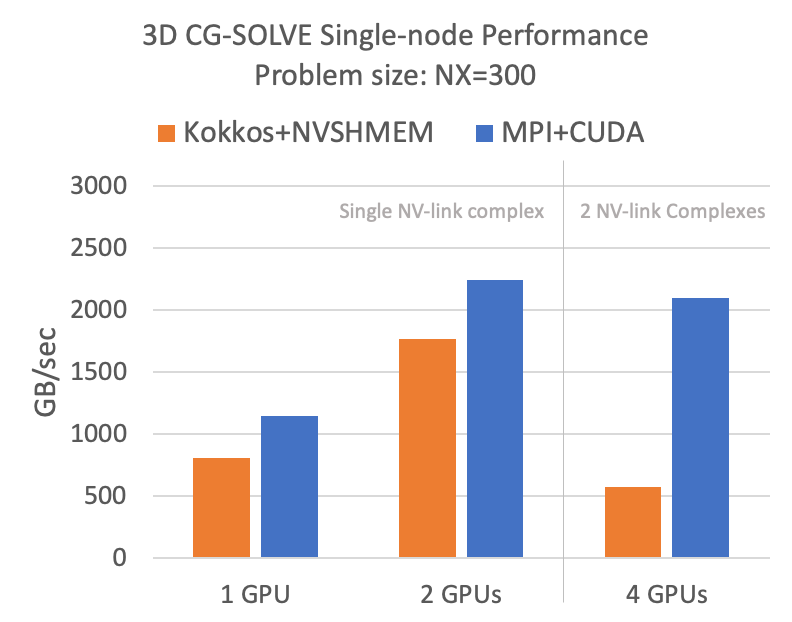
\includegraphics[width=0.99\textwidth]{figures/PGAS_CGSolve_Perf}
    \end{center}
    \column{.5\textwidth}
    \begin{center}
      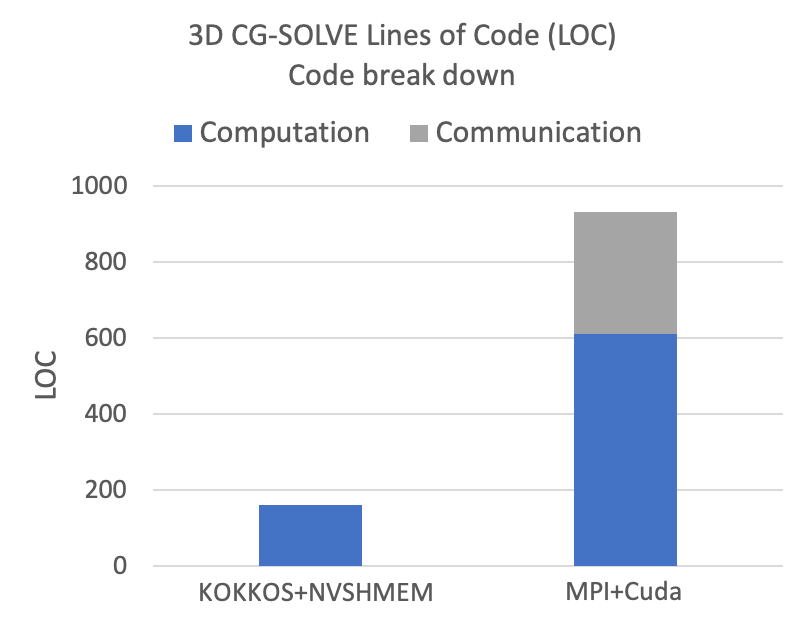
\includegraphics[width=0.99\textwidth]{figures/PGAS_CGSolve_LOC}
    \end{center}
  \end{columns}
\end{frame}

%=============================================
%=============================================
%=============================================

\begin{frame}{Remote Spaces: Code and Configuration}
  \vspace{6pt}
  \textbf{Get it on GitHub}
  \begin{itemize}  
  \item\url{https://github.com/kokkos/kokkos-remote-spaces}
  \end{itemize}
  \vspace{6pt}
  \textbf{Configuration Example}
  \begin{itemize}
    \item\textbf{NVSHMEM}: \small\texttt{cd \$(kokkos\_remote\_spaces) \\
  cmake . -DKokkos\_DIR=\$(KOKKOS\_HOME)/install -DCMAKE\_CXX\_COMPILER=mpicxx  -DNVSHMEM\_ROOT=\$(NVSHMEM\_HOME)/install -DKokkos\_ENABLE\_NVSHMEMSPACE=ON}
  \item\textbf{SHMEM}: \small\texttt{-DKokkos\_ENABLE\_SHMEMSPACE=ON}
  \item\textbf{MPI One-Sided:}\small\texttt{-DKokkos\_ENABLE\_MPISPACE=ON}
  \end{itemize}
  \vspace{8pt}
  % \begin{block}{Important Point}
    \textbf{Note:} Setting the \texttt{-DKokkos\_ENABLE\_\{SPACE\}} CMAKE flag sets \texttt{Kokkos::Experimental::DefaultRemoteMemporySpace} to the given \textbf{PGAS backend}.
  %\end{block}
\end{frame}

%=============================================
%=============================================
%=============================================

\begin{frame}[fragile]{Exercise: Vector-Shift}
\textbf{Exercise: Implementing a Distributed Vector-Shift}
  \vspace{10pt}
  \begin{itemize}
    \item Location: \ExerciseDirectory{pgas\_vectorshift}
    \item Compile and run with one and two ranks using SHMEM (CPUs) or NVSHMEM (GPUs)
  \end{itemize}
  
  \begin{code}
    mkdir build && cd build
    cmake . -DKokkosRemote_ROOT=<path-to-Kokkos-Remote-Spaces>/install -DCMAKE_CXX_COMPILER=mpicxx
    cmake .. && make
    # Run exercise
    mpiexec -np 2 ./vectorshift
  \end{code}
\end{frame}

%=============================================
%=============================================
%=============================================

\begin{frame}{Remote Spaces: Summary}
\textbf{Summary: Kokkos Remote Spaces}
\vspace{10pt}
\begin{itemize}
   \item Adds distributed shared memory to Kokkos.
   \item View-templating defines memory space (SHMEM, NVSHMEM or MPI One-Sided).
   \item View \texttt{()-operator} implements the \texttt{Put/Get semantic}.
   \item Use \texttt{deep\_copy(...)} to move data between memory spaces.
\end{itemize}
\end{frame}

%=============================================
%=============================================
%=============================================
